Before starting the development of the project, research shown that a few prototypes are currently in development with similar specifications. These projects present a variety of functionalities but due to the simplicity of the systems, all of them are addressed to educational field. The three projects analysed present some different strengths and weaknesses. 

In the case of Pi-Bot \cite{PiBot} project, the current version of the platform includes and Arduino board which reduces dramatically the computational power, fact that does not allow camera features unless the system is upgraded to a Raspberry Pi board. However, seems to be the most friendly and better design platform due to the simplicity and guidance of the development environment.

Another two remarkable projects currently on the field based on Raspberry Pi using PiCamera and wireless connection are GoPiGo \cite{GoPiGo} and TiddlyBot \cite{TiddlyBot}. On one hand, GoPiGo project is a complete kit that turns the Pi into a fully operating robot open for developers but it does not provide any functionality more than the hardware itself. It provides more freedom and space for the creativity although it is not suitable for beginners.

On the other hand, TiddlyBot is a little bit more complete. For instance, the software package provides some amazing features such as draws, follow lines, and helps with the learning of technology. Additionally, it is possible to drive round your house using a tablet, smartphone or computer streaming the Pi's camera back to your device.

\begin{figure}
     \centering
     \begin{subfigure}[b]{0.3\textwidth}
             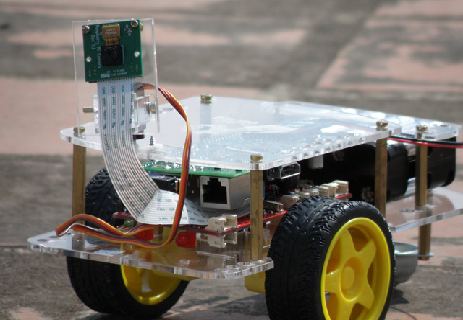
\includegraphics[width=\textwidth]{GoPiGo.png}
             \caption{GoPiGo}
             \label{fig:GoPiGo}
     \end{subfigure}%
     ~
     \begin{subfigure}[b]{0.3\textwidth}
             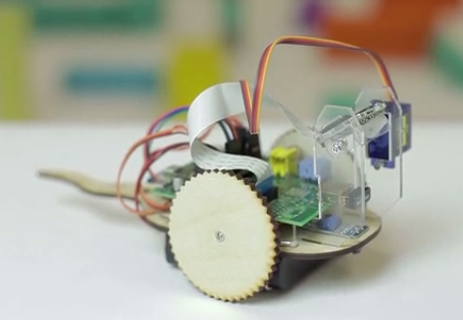
\includegraphics[width=\textwidth]{TiddlyBot.png}
             \caption{TiddlyBot}
             \label{fig:TiddlyBot}
     \end{subfigure}
     \caption{Similar educational robots}\label{fig:robots}
\end{figure}